\chapter{Конструкторская часть}

В данном разделе будут представлены схемы реализации алгоритма обратной трассировки лучей, его однопоточной и многопоточной реализаций.

\section{Разработка алгоритма обратной трассировки лучей}
На рисунке \ref{img:raytrace} представлена схема реализации алгоритма обратной трассировки лучей.

\begin{figure}[h!]
    \centering
    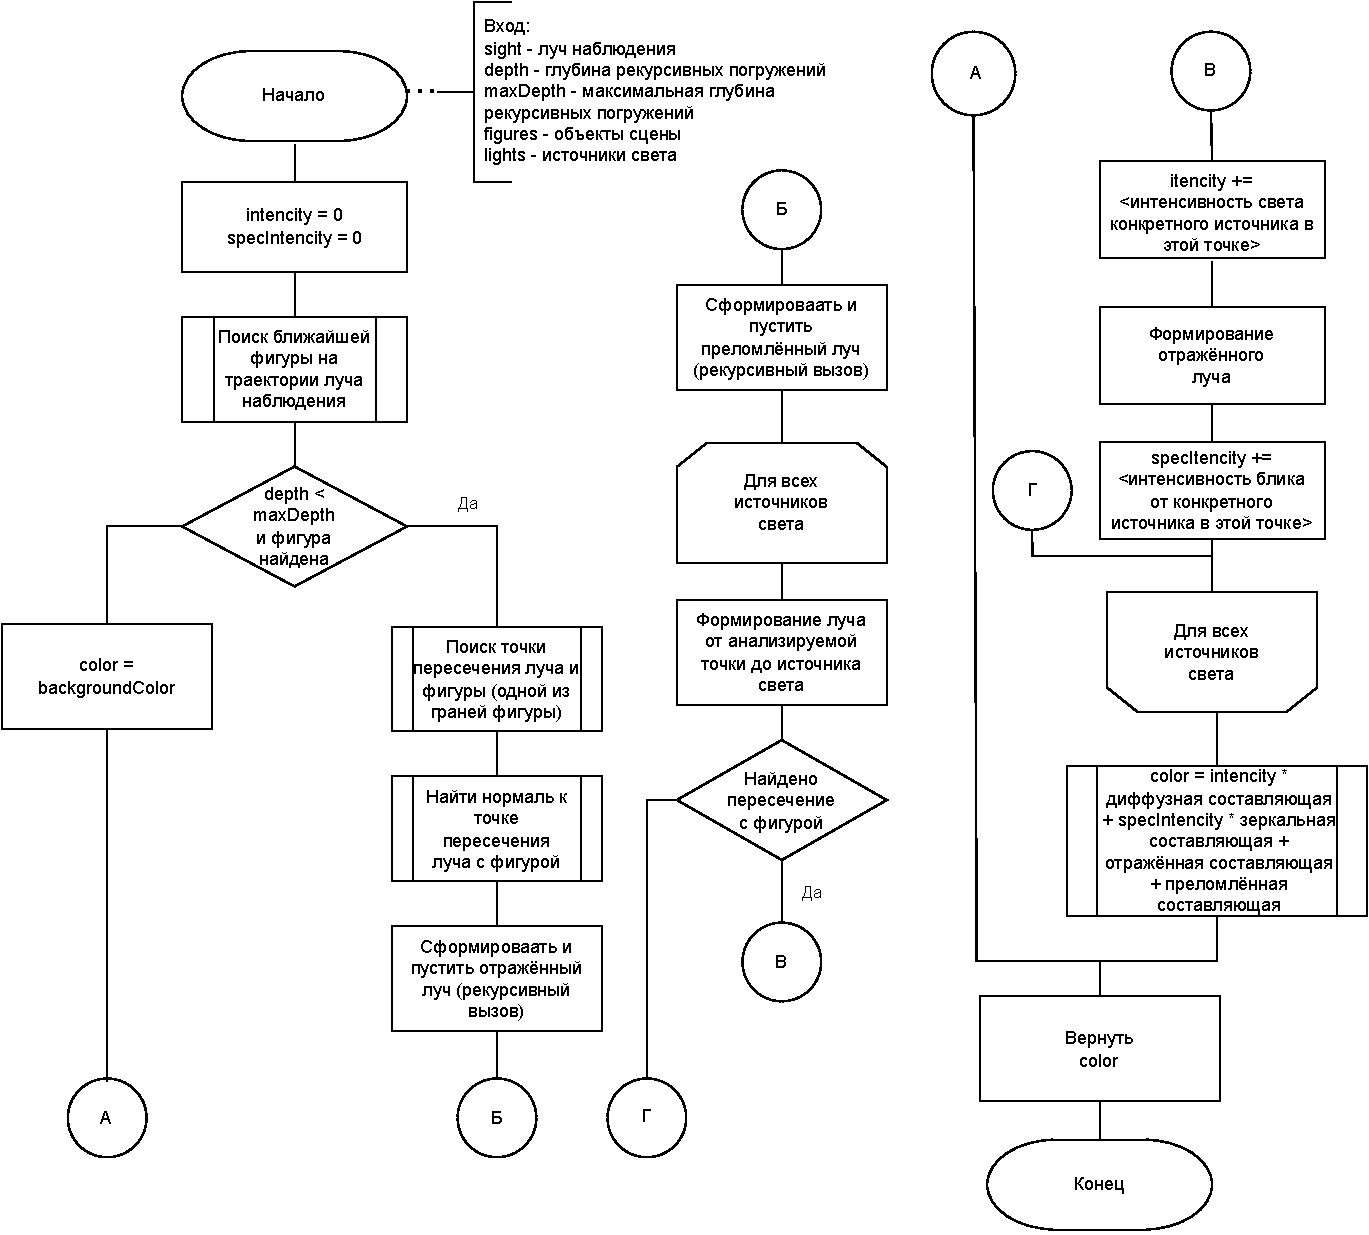
\includegraphics[width=1\linewidth]{raytrace.pdf}
    \caption{Схема реализации алгоритма обратной трассировки лучей}
    \label{img:raytrace}
\end{figure}

\section{Разработка последовательного алгоритма обратной трассировки лучей}
На рисунке \ref{img:one} представлена схема последовательного алгоритма обратной трассировки лучей.

\begin{figure}[h!]
    \centering
    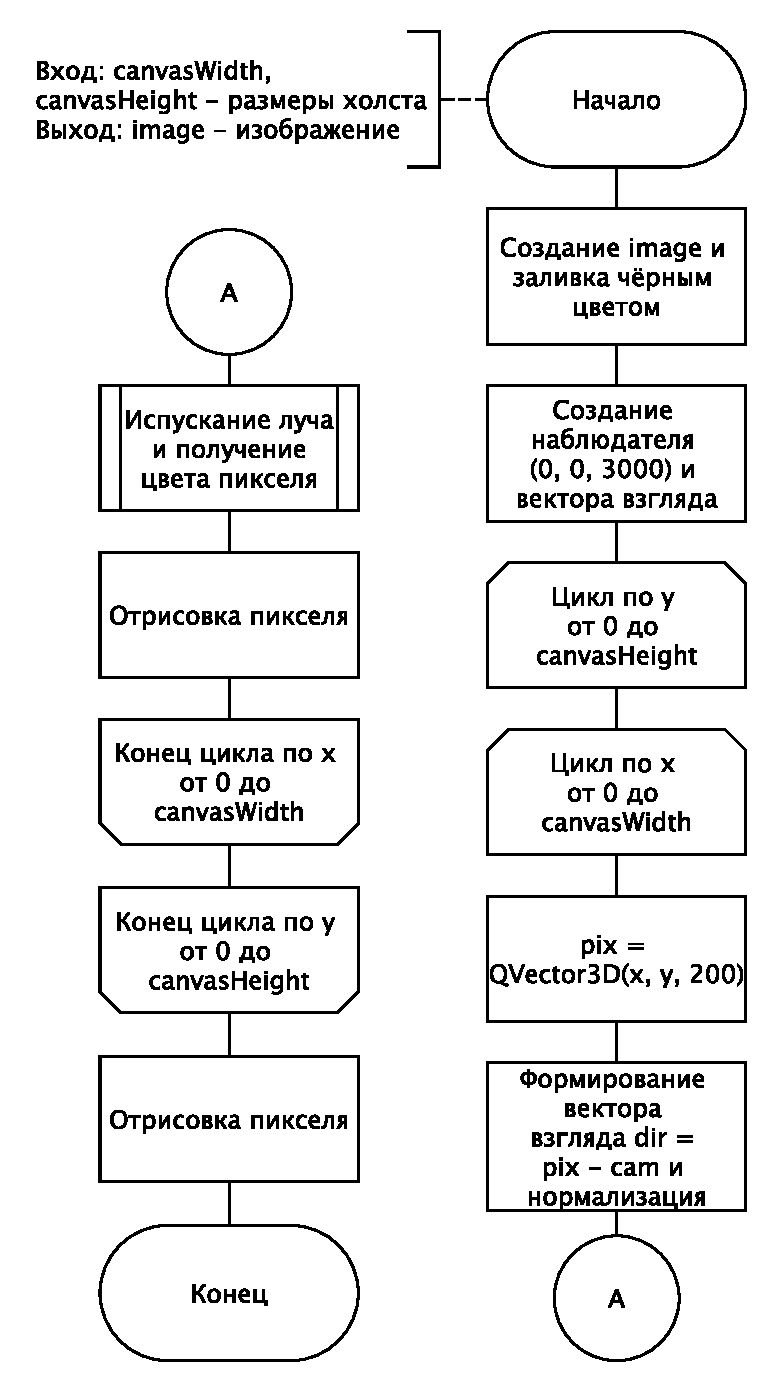
\includegraphics[width=0.6\linewidth]{one.pdf}
    \caption{Схема последовательного алгоритма обратной трассировки лучей}
    \label{img:one}
\end{figure}

\section{Разработка параллельного алгоритма обратной трассировки лучей}
На рисунке \ref{img:many} представлена схема параллельного алгоритма обратной трассировки лучей.

\begin{figure}[h!]
    \centering
    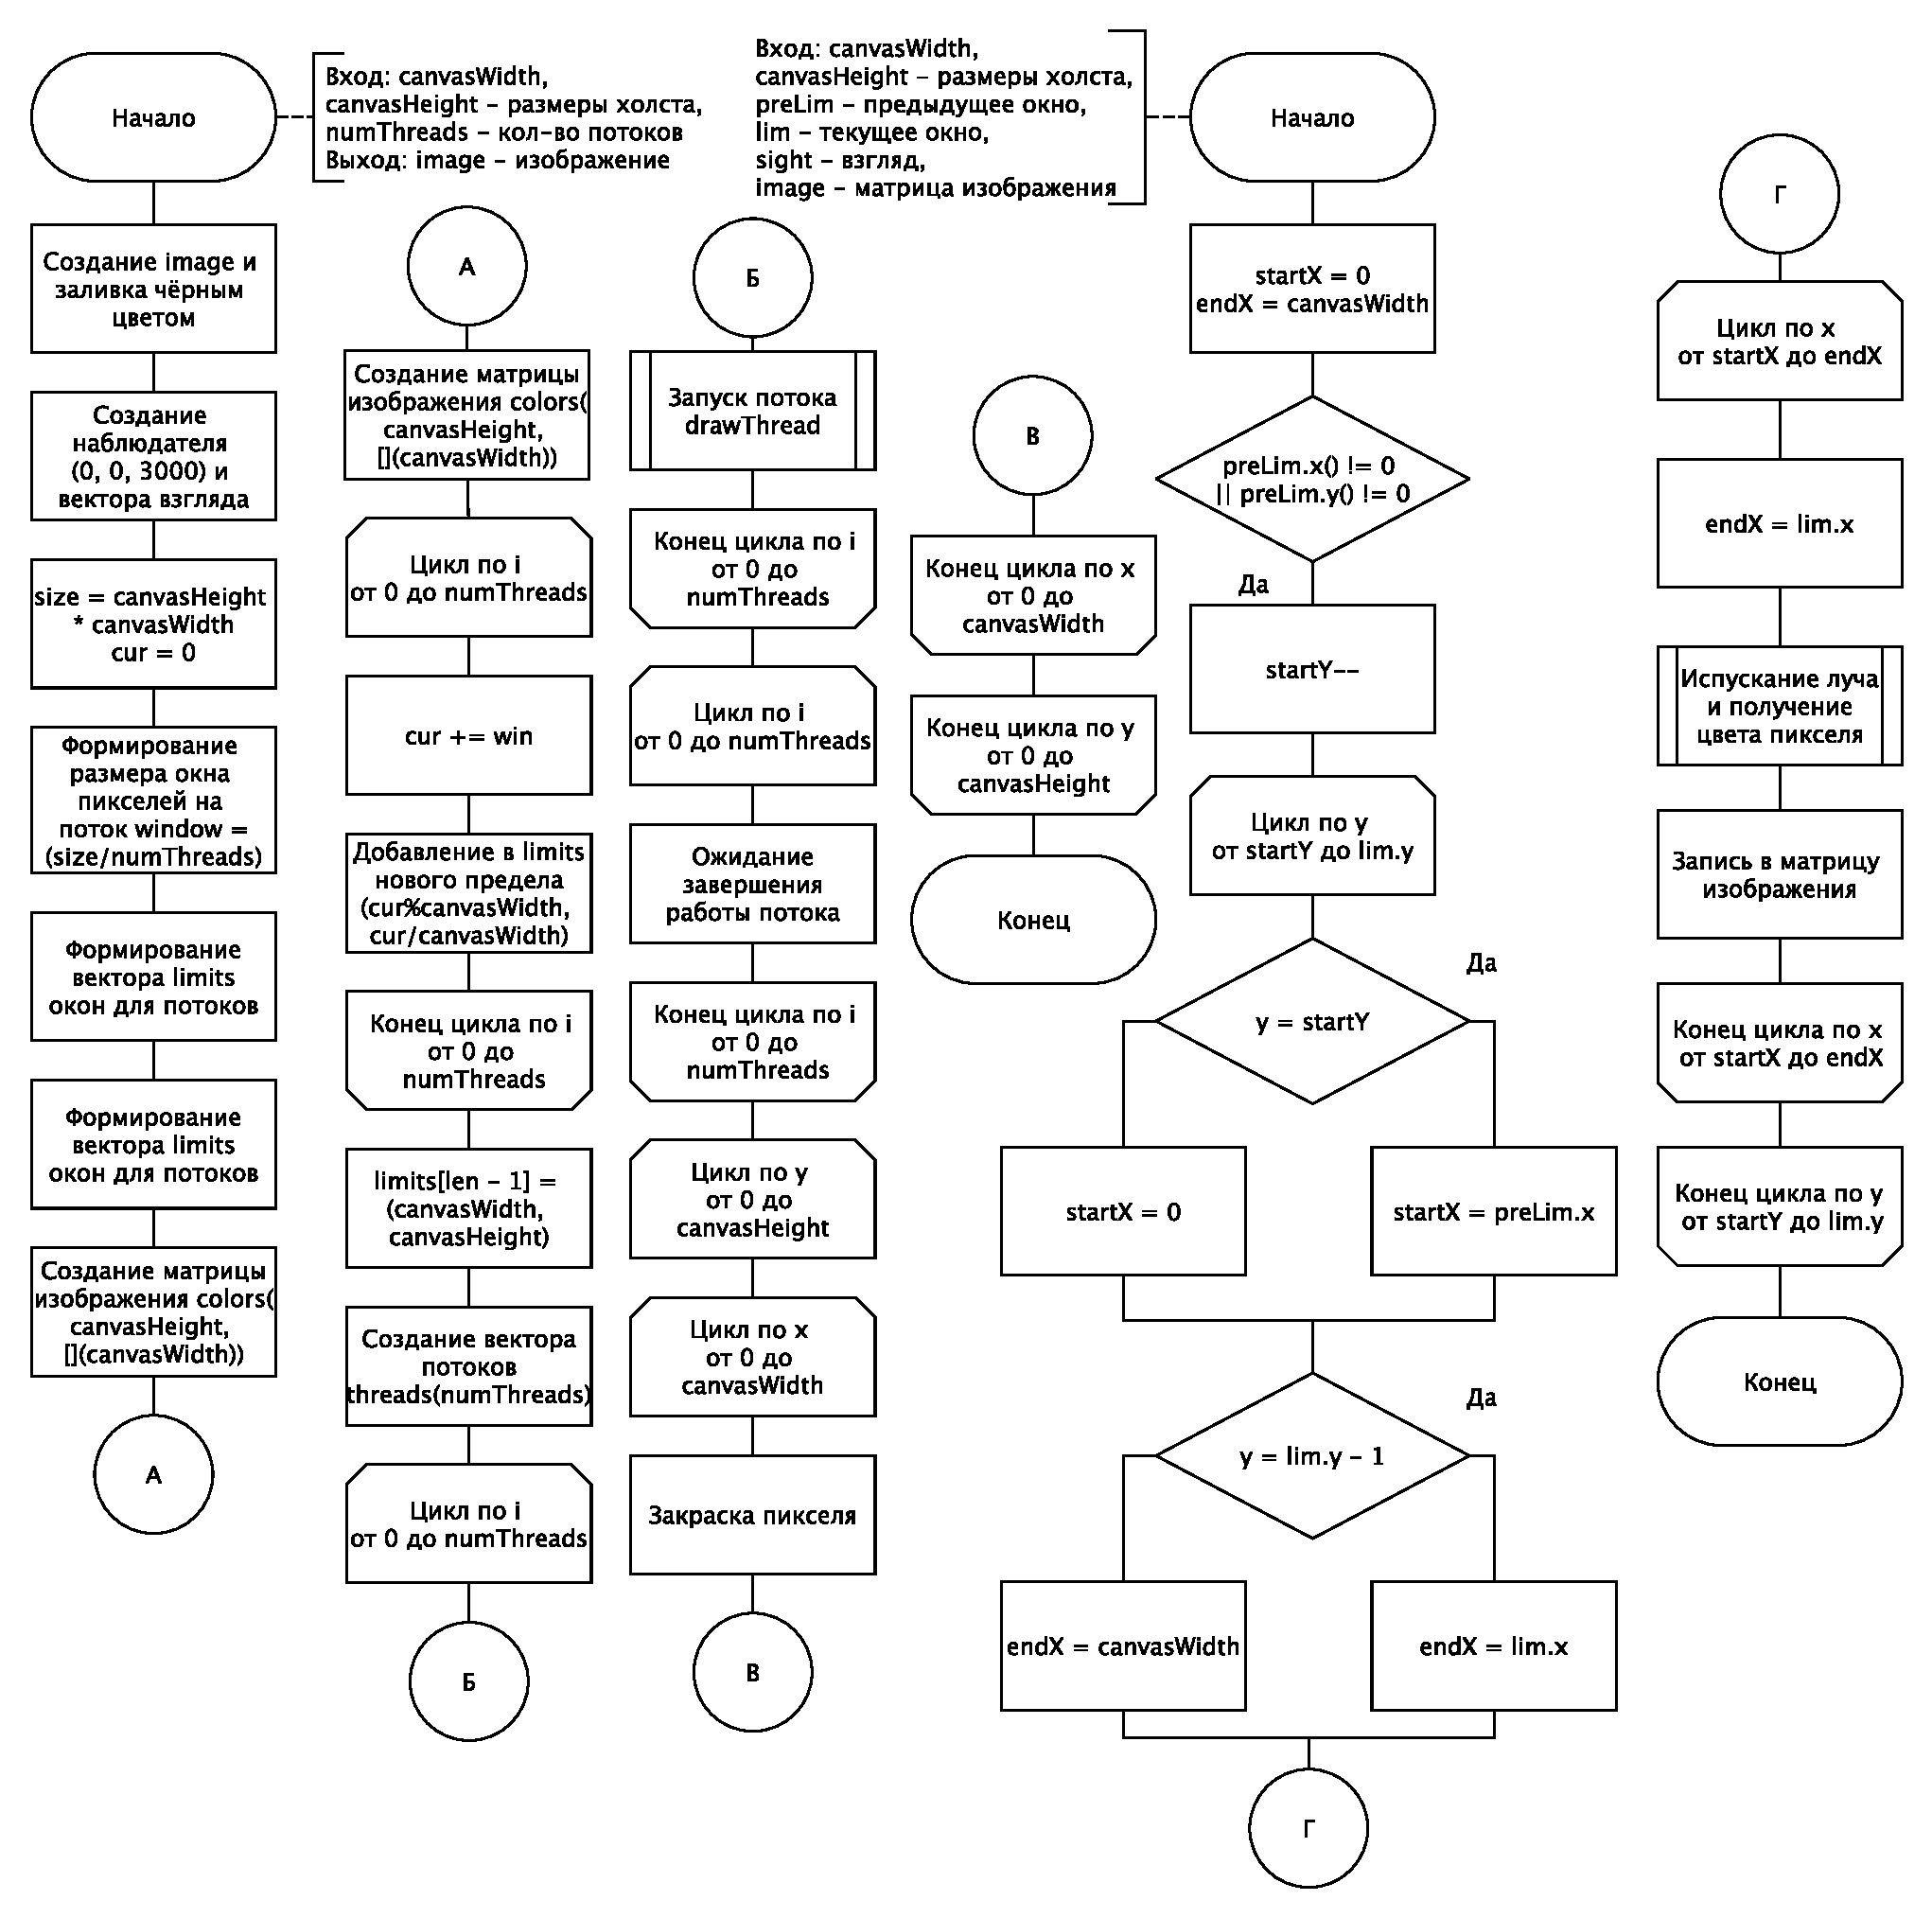
\includegraphics[width=1\linewidth]{many.pdf}
    \caption{Схема параллельного алгоритма обратной трассировки лучей}
    \label{img:many}
\end{figure}

\newpage